\subsection{SVM parameter tuning}
\label{sec:imk}
%Recall in section \ref{sec:tree} we consider a user $u_i$ as a opinion leader if $followers_i/friends_i>\alpha$.
%The larger the $\alpha$ is, the less the user will be considered as a opinion leader.
The SVM classifier is implemented using LIBSVM\cite{LibSVM}.
We first use the small data set and 10-fold cross validation to
obtain the following parameters values that will be used in
all subsequent experiments:
\begin{eqnarray*}
2\sigma^2 &=& 3 \\
\rho &=& 0.1 \\
\gamma &=& 2^{-11} \\
cost &=& 2^{13}
\end{eqnarray*}

By Eq. (\ref{eq:alpha}), $\alpha$ controls the number of opinion leaders
in the tree and hence affects the final simplified tree and the
calculation of the kernel function.
Here we analyze the impact of $\alpha$ on the size of the product graph
in the graph kernel as well as the accuracy of the
SVM through 10-fold cross validation.
%to evaluate the performance of SVM classifier and the average number
%of vertices of $A_\times$ to measure the size of simplified graph.
To suppress the effects of the vector kernel, we set $\beta=1$ in this
experiment.
%Since the calculation is time-consuming, we did the
%experiment on a randomly selected data set with 500 rumors and 500 non-rumors.
The results of experiment are shown in \figref{fig:result-alpha-size} and
\figref{fig:result-alpha-accuracy}.
\begin{figure}[htb]
\centering
\includegraphics[height=120pt]{impact_alpha_size.eps}
\caption{Average number of vertexes in product graph vs. $\alpha$}
\label{fig:result-alpha-size}
\end{figure}
\begin{figure}[htb]
\centering
\includegraphics[height=120pt]{impact_alpha_accuracy.eps}
\caption{Classification accuracy vs. $\alpha$}
\label{fig:result-alpha-accuracy}
\end{figure}

Accuracy hits the maximum when $\alpha = 20$.
%When $\alpha$ is larger than 20 the accuracy of SVM classifier decreases.
It is also interesting to note that as $\alpha$ grows, the size of the graph
converges, which indicates that when $\alpha$ is large, most ordinary users
have been merged into super nodes and there are only small number of
opinion leaders in the ``long tail'' who have extremely large fan base.
%Besides, when $\alpha$ becomes large enough, the size of graph is decreasing slowly. This is because that when $\alpha$ is very large, the users that still be considered as opinion leaders are the ``superuser'' whose followers are much more than friends.
In the following experiments, we set $\alpha = 20$.

%In section \ref{sec:combined} we define the combined kernel function as the sum of random walk kernel and vector kernel. There is a parameter $\beta$ that rules the contribution of random walk kernel.
Next we try to tune the best $\beta$ value to balance the graph kernel and
the RBF kernel.
%The whole data set is divided into training set and test set,
%the ratio of two sets is 2:1.
For each value of $\beta$, we train an SVM classifier
and record its accuracy. The results of experiment are shown in
\figref{fig:result-beta}.
\begin{figure}[htb]
\centering
\includegraphics[height=120pt]{impact-beta.eps}
\caption{Accuracy, F$_1$ for false rumors and for other messages vs. $\beta$}
\label{fig:result-beta}
\end{figure}

Results show that when $\beta=0.6$, the hybrid kernel achieves the best accuracy
and the combination of the two kernels performs better than each individual
kernel (two ends of the graph). Therefore, in the following experiments,
we set $\beta = 0.6$.
